\chapter{The ATLAS Experiment}\label{sec:atlas}
Exploring the nature of the Higgs particle requires collision energies on the \qty[]{}{TeV} scale. With the \ac{lhc} as the most powerful particle accelerator currently in existence making it the the premier facility for studying the Higgs particle. The main reference for this section is \citep{aad2008atlas}.

\section{The Large Hadron Collider}
The \ac{lhc} is a circular proton proton collider with \qty[]{27}{km} circumference with a center-of-mass energy of $\sqrt{s}=\qty[]{13}{TeV}$. The two anticyclic proton beams comprise several bunches that contain $10^{11}$ protons. These bunches are brought to collisions at several points along the ring facilitating various experiments conducted at the LHC. A measure of how tightly particles are packed in these bunches is the instantaneous luminosity and is characteristic to the collider
\begin{equation}
    L=\frac{1}{\sigma}\frac{\dint{N}}{\dint{t}}.
\end{equation}
It can be read as particle interactions per unit time and area. The area understood as the interaction cross-section of a particular process. The total recorded number of collision events can thus be calculated by summing the luminosity over time which gives with the integrated luminosity
\begin{equation}
    N=\sigma\cdot\int L dt=\sigma\cdot L_\mathrm{int}.
\end{equation}
For the full run 2 dataset used in this thesis the integrated luminosity for events good for physics analysis is \qty[]{140.1}{fb^{-1}} \citep{DAPR-2021-01}.

\section{The ATLAS detector}
The \ac{atlas} (A Toroidal LHC Apparatus) experiment is a particle detector with an onion-like structure, as shown in figure \ref{fig:atlas_detector}.
\begin{figure}
    \centering
    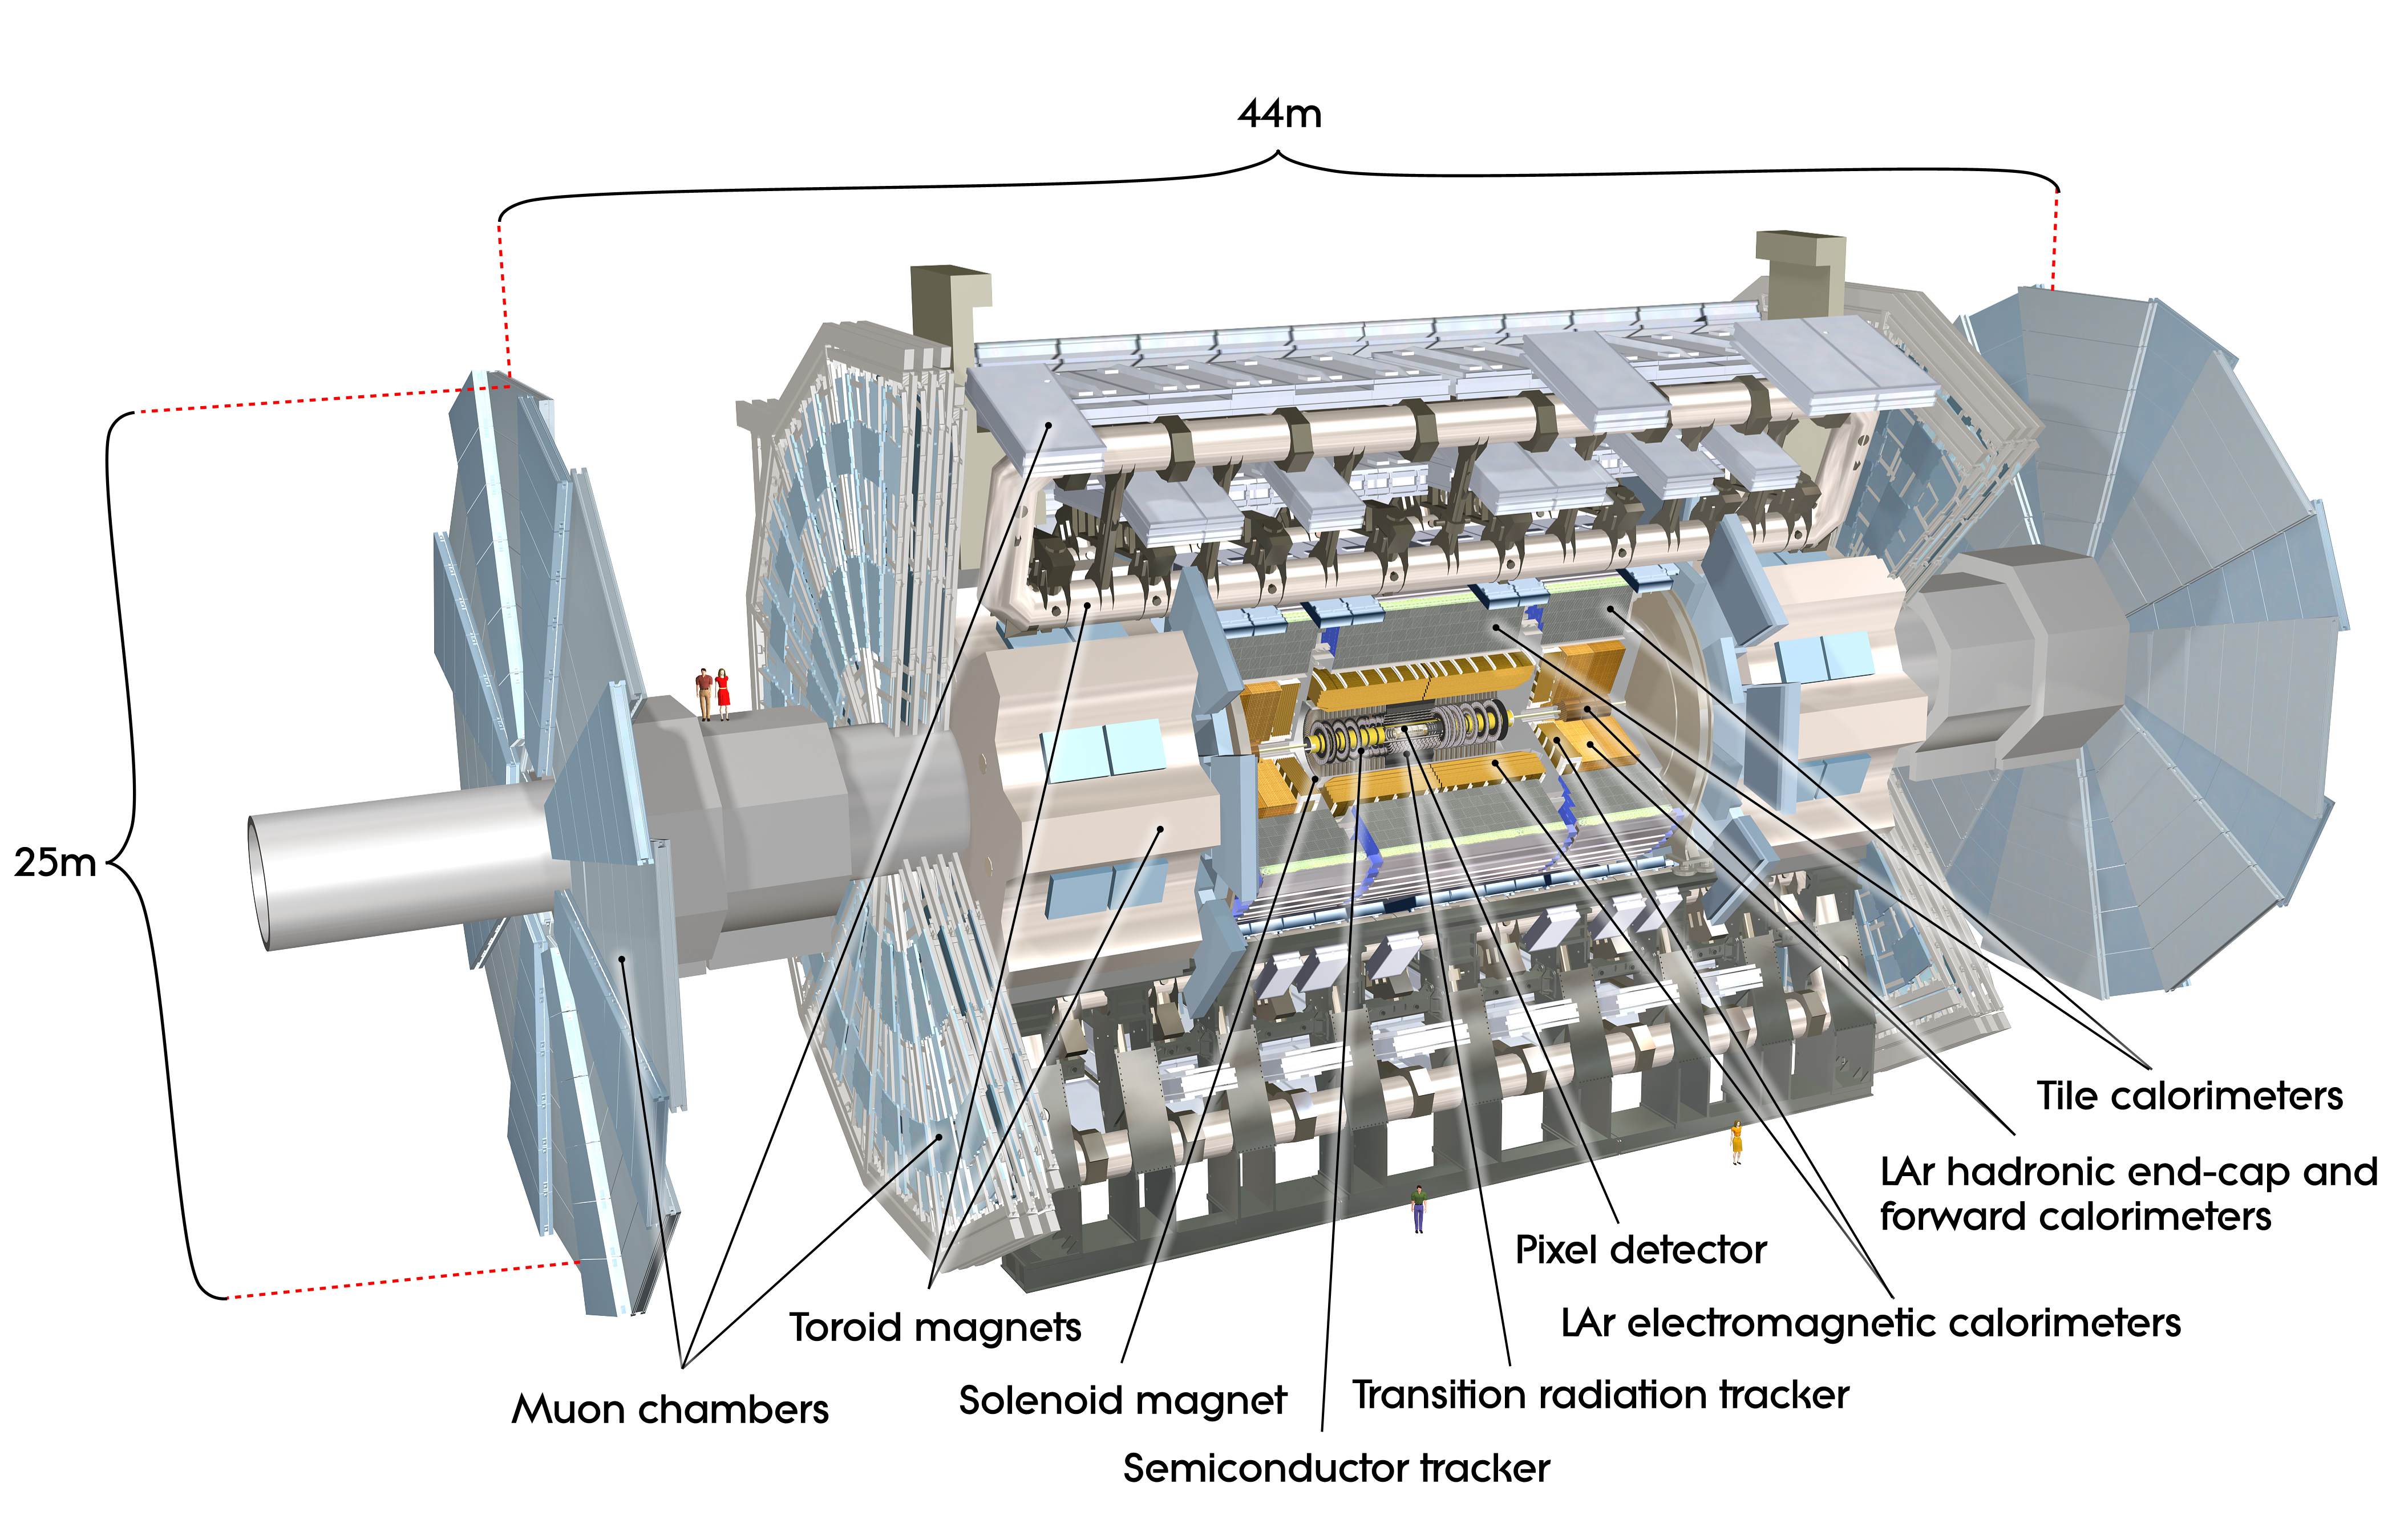
\includegraphics[width=1\textwidth]{atlas_detector}
    \caption[]{The \ac{atlas} experiment at the \ac{lhc} with its subdetectors. Adopted from \citep{Pequenao:1095924}.}
    \label{fig:atlas_detector}
\end{figure}
Its purpose is to measure the trajectory, momentum, and energy of particles originating from proton-proton collisions, depending on the particular kind of interaction of the collision products with matter. The various subdetectors are explained below from the inside out.

\subsection*{Coordinate System}
The coordinate system of \ac{atlas} is right-handed and originates at the interaction point at the center of the detector. The z-axis points along the beam line, the x-axis to the center of the \ac{lhc} and the y-axis away from earth. Quantities transversal to the z-axis are therefore Lorentz-invariant. Inside the detector cylindrical coordinates $r,\phi$ are used with $\phi$ the azimuthal angle about the z-axis. The polar angle $\Theta$ of a particle is expressed through the pseudorapidity $\eta=-\ln(\Theta/2)$. This quantity is defined as an approximation for the Lorentz invariant rapidity and holds for highly relativistic particles. This provides a valuable measure for describing angular separation $\Delta R$ between objects within the detector
\begin{equation}
    \Delta R = \sqrt{(\Delta\phi)^2+(\Delta \eta)^2}.
    \label{eq:delta_R}
\end{equation}

\section{Inner Detector}\label{sec:inner_detector}
The inner detector, shown schematically in figure \ref{fig:inner_tracker}, is designed to track charged particles and to determine their momentum and to provide insights into their particle type.
\begin{figure}
    \centering
    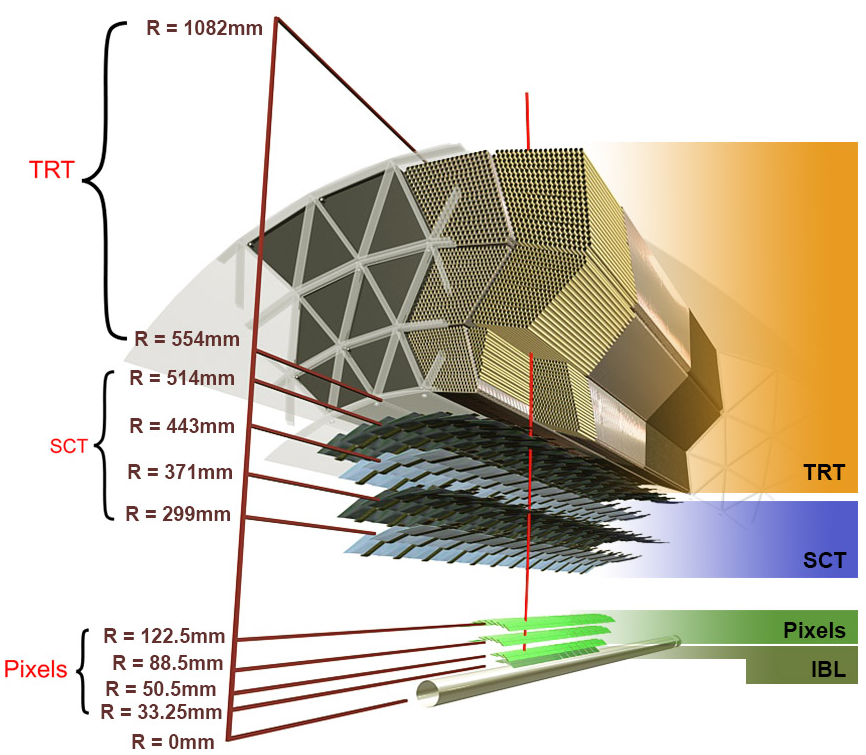
\includegraphics[width=0.65\textwidth]{inner_tracker}
    \caption[]{The inner detector schematically with the subdetectors described in the full text. Adopted from \citep{Potamianos:2016ptf}.}
    \label{fig:inner_tracker}
\end{figure}
It is surrounded by a solenoid magnet whose field lines point in the direction the beam so that charged particles are bent in the transverse plane of the detector due to the Lorentz force. The direction of this bending reveals the particle's charge while the degree of curvature relates directly to its momentum.

The \ac{ibl}, pixel detector, and \ac{sct} consist of silicon detectors of various sizes. When passing through silicon, charged particles ionize electrons that travel in an electric field to an electrode and provide positional information. The \ac{ibl} plays a crucial role in b-tagging as will become clear in section \ref{sec:b_tagging}.

Aforementioned semiconductor trackers are surrounded by the \ac{trt} which assist further in tracking and identification of particles. It consists of multiple layers of tubes arranged perpendicular to the beamline. These tubes are filled with a gas mixture and have a conducting wire at their center, maintained under a voltage to attract negatively charged particles. The tubes are surrounded by a material with different permittivity so that charged particles traversing these materials emit transition radiation. The intensity of this radiation depends on the velocity, making it possible to distinguish between particles of different types. For instance, for particles with the same energy, lighter ones like electrons emit more photons compared to heavier particles like pions, aiding in their identification.

\section{Calorimeters}\lab{sec:calorimeters}
When high-energy particles pass through dense matter they interact with the matter through various processes such as ionization and excitation, bremsstrahlung, pair creation and annihilation, or by interacting with the nuclei of the material. These interactions result in the creation of secondary particles which then generate a particle shower. By reconstructing this shower, the energy of the particles can be inferred. In the \ac{ATLAS} detector, this is achieved using two sampling calorimeters. These calorimeters consist of alternating layers: a high-density metal that absorbs the energy of the particles and a material capable of tracking these particles.

\subsection{Electromagnetic Calorimeter}

In the electromagnetic calorimeter the main energy deposits are from electrons and photons. The stopping material consists of lead and steel and is alternated with a copper plate on which there is an electrode grid. Between the plates is liquid argon. When interacting with the dense metal e.g. by bremsstrahlung of an electron or by pair production induced by a photon, the created secondary particles ionize the argon atoms in between. The negatively charged ions are then pulled to the charged copper electrodes to determine the position. From the distance a particle has traveled through the electromagnetic calorimeter the energy of the particle can be inferred.

\subsection{Hadronic Calorimeter}

Hadrons also deposit energy in the electromagnetic calorimeter but interact with nuclei as well. However as they are more energetic more stopping power is needed which is provided by the hadronic calorimeter that surrounds the electromagnetic calorimeter. The configuration is made of many layers of tiles positioned in planes perpendicular to the beamline. In these layers tiles of steel as stopping material alternate by a scintillating plastic which radiates light if charged particles pass through. The light is collected at the edges by wavelength-shifting optical fibres  which reduce the energy of the photons and then read out by photomultiplier tubes.

\section{Muon Spectrometer}

The muon spectrometer encircles all other detectors to capture muons which barely loose energy passing through the other detectors. The core elements of the muon spectrometer are resistive plate chambers, arranged in three layers around the calorimeters. Essentially functioning as charged capacitors filled with gas, these chambers detect charged particles when they ionize the gas inside. The resultant ion avalanche, attracted to the electrodes, is then measured to determine the particle's position. Additionally, the detection process is enhanced by electrodes, akin to those in the \ac{TRT}, comprising tubes filled with gas and a central wire.

Figure \ref{fig:particles_in_detector} illustrates the interaction of different particle types with the various sections of the particle detector. 
\begin{figure}
    \centering
    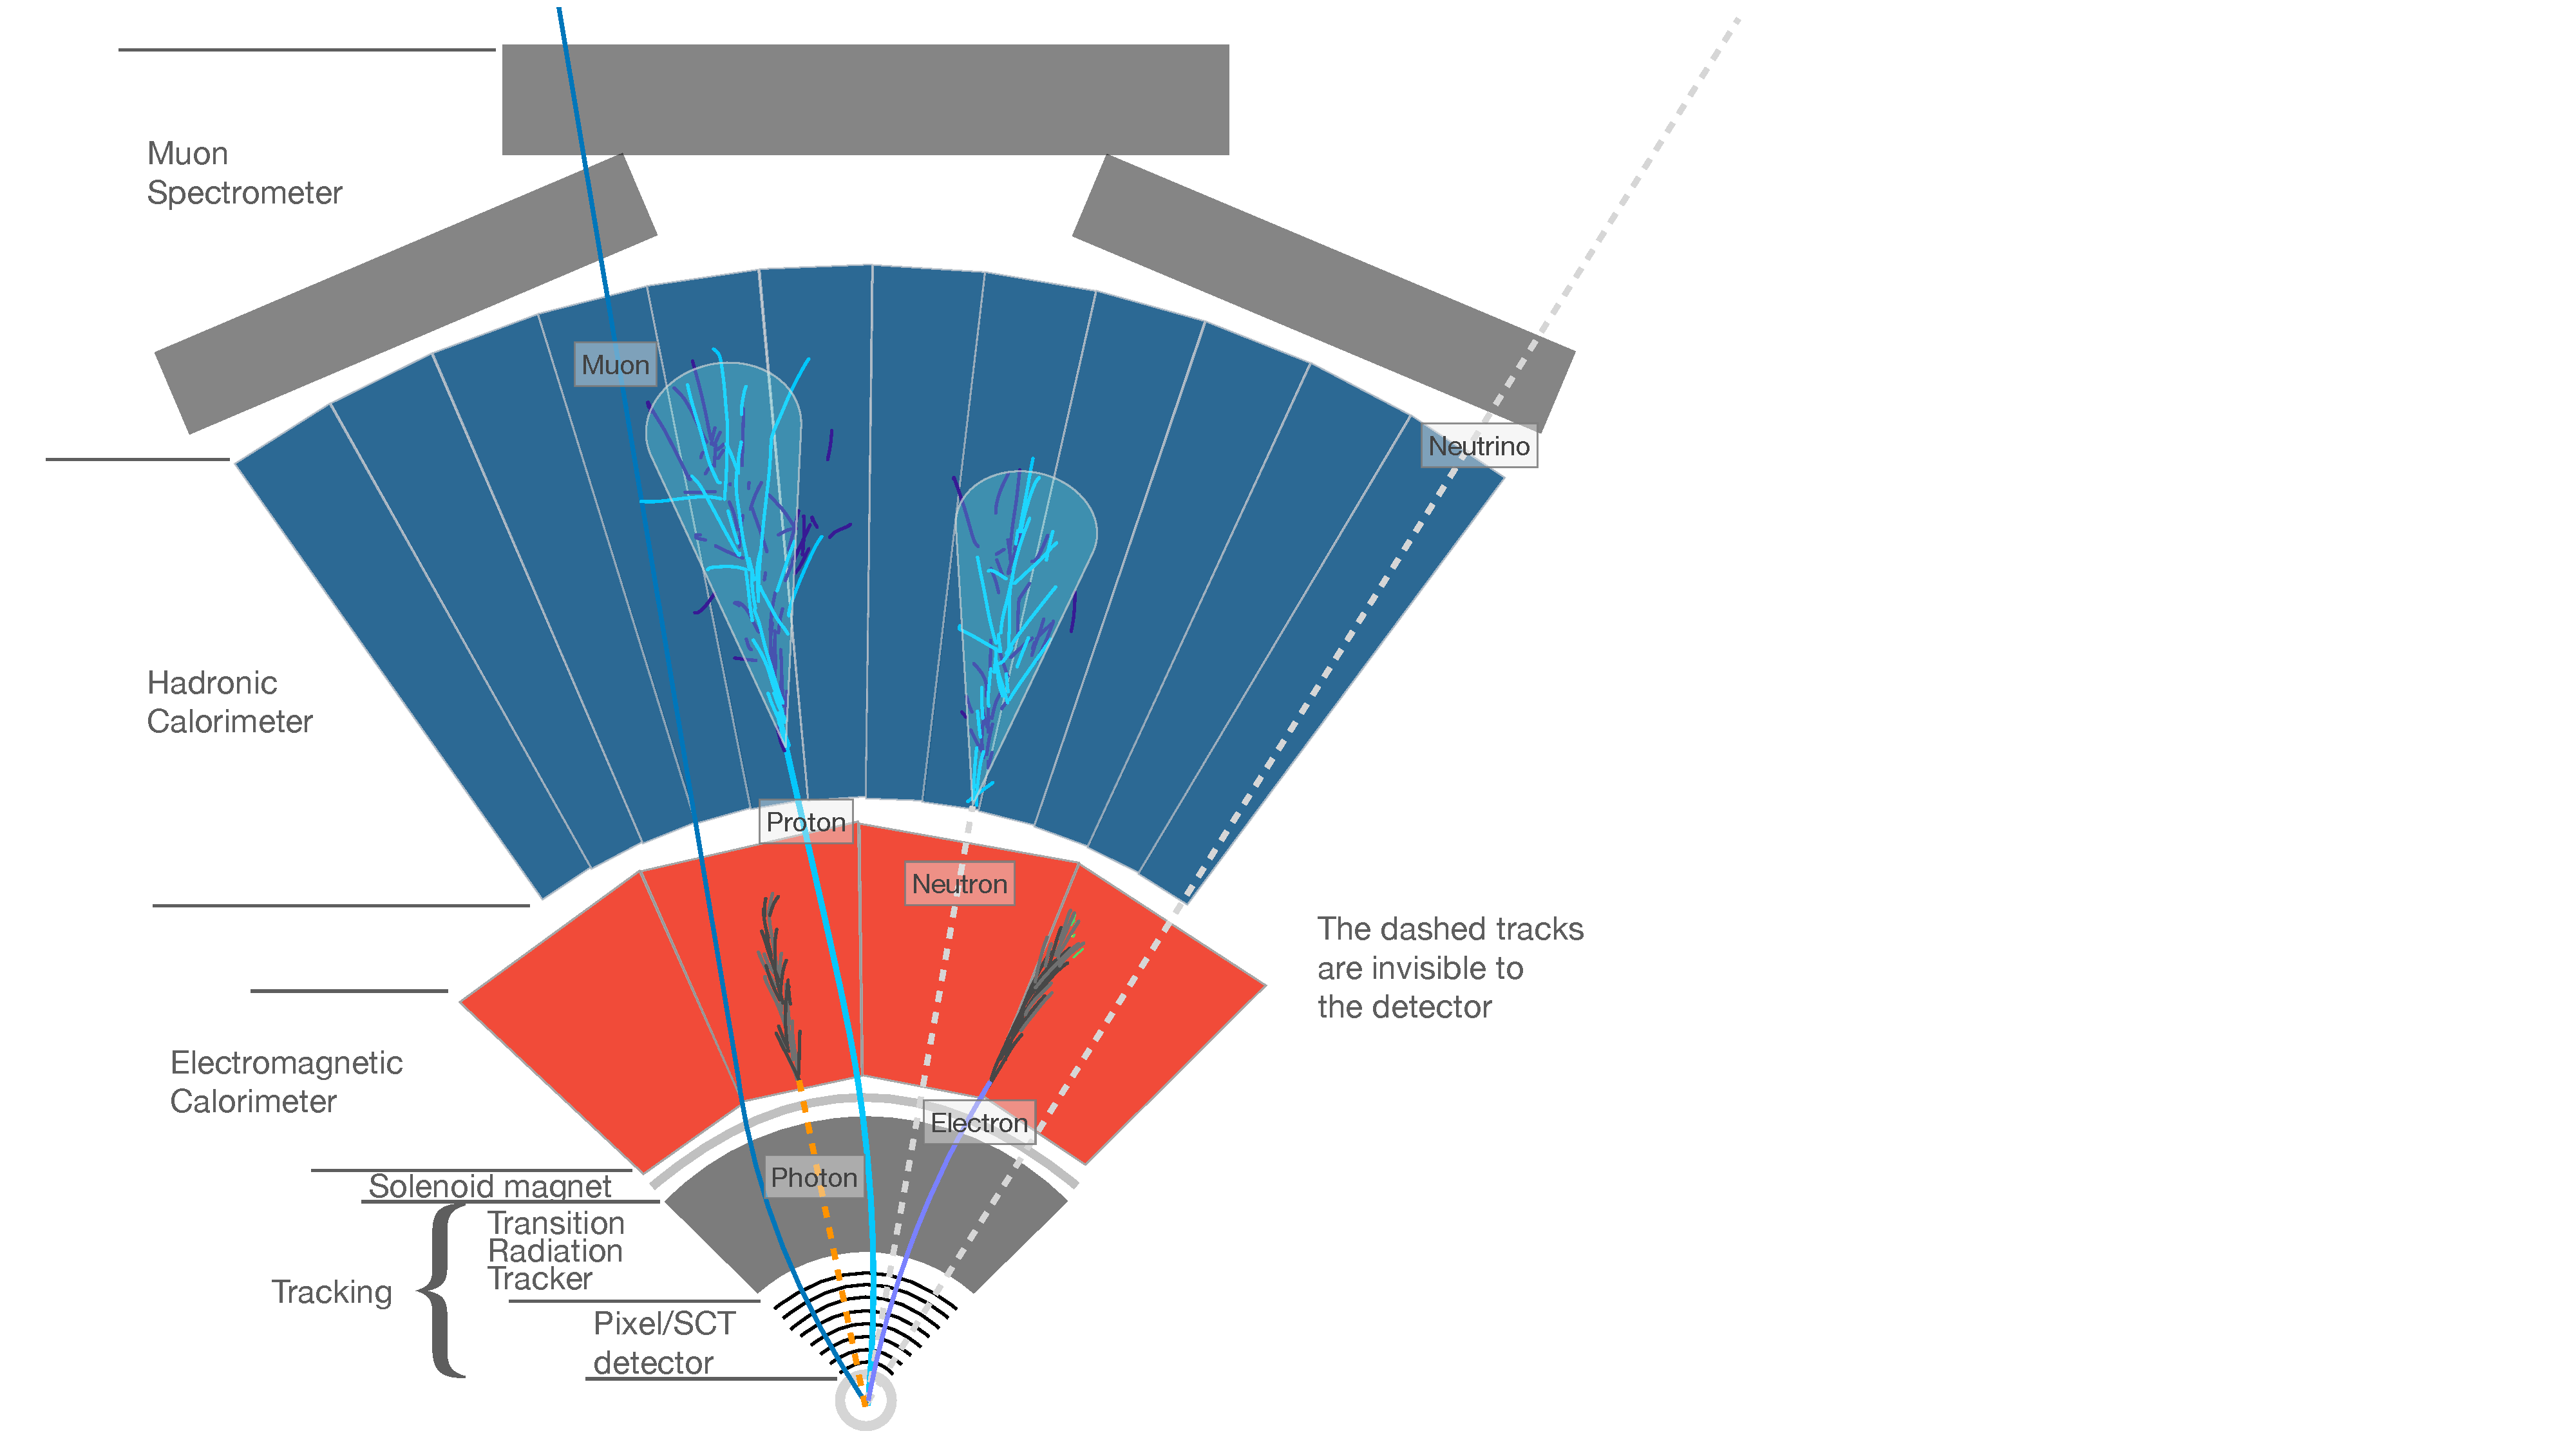
\includegraphics[width=1\textwidth]{particle-shower}
    \caption[]{Paths and energy deposits of particle types in the subdetectors. Adopted from \citep{Guth:2765038}.}
    \label{fig:particles_in_detector}
\end{figure}

\section{Data Acquisition}\label{sec:tdaq}
In the \ac{LHC}, bunches of protons are collided within the \ac{ATLAS} detector at a rate of 40 MHz. Currently, it is technically infeasible to record all these collisions, as doing so would require handling a data rate of approximately 40 TB/s. To manage this, a preselection process known as triggering is employed, which is carried out in two stages.

The first stage is the hardware-based \ac{L1} trigger, which reduces the event rate to about 100 kHz. This reduction is achieved by selecting events that exhibit large transverse momentum deposits in the detector or those that have missing transverse momentum. The regions in the detector where these criteria are met are then passed to a software-based \ac{HLT}. The \ac{HLT} then uses the full detector information in these regions to reduce the rate further down to \qty[]{1}{kHz}.
